\section[Check for understanding: More Vectors]{Check for understanding: Force, Velocity, and Momentum Vectors}
\label{act6.1.3b}
\note{For Activity~\ref{act6.1.3b} (\about\unit[40]{min})}{
In  small groups, Compare  responses to \FNT~\thechapter-\ref{fnt6.1.2-4} through \thechapter-\ref{fnt6.1.2-7} and \FNT~\thechapter-\ref{fnt6.2.1-1} with other members of your small group.  Come to a consensus on an appropriate response to each \FNT{} and be able to make convincing reasons why you know for sure your response is appropriate.  Each person in your group should be prepared to do this for any of the \FNTs.  Nothing on board
Whole Class Sharing
}

\begin{overview}

\textbf{Overview:} In this section, we'll practice what we've learned about force and velocity vectors, so far.

\end{overview}

\note{for \FNT~\thechapter-\ref{fnt6.1.2-4} }{
$\vec{F}_{1} = (-4, 2)$; $\vec{F}_{2} = (8, 9)$;  $\Sigma \vec{F} = (-8, 0)$
\\[0.25in]
Answer should be found graphically:
Solution: $\vec{F}_{3} $ = (-12, -11)
}
\begin{FNTenv}
	\label{fnt6.1.2-4}

\begin{wrapfigure}{R}{0.5\textwidth}
	\vspace{-35pt}
	\begin{center}
	\begin{tikzpicture}[thick,scale=0.65, every node/.style={transform shape},background rectangle/.style={fill=white}, show background rectangle]
		% draw a 10x7.5 grid in light gray with 5mm grid spacing
		\draw[step=.5cm,gray,very thin] (0,0) grid (10,7.5);
		% draw a darker grid in light gray with 2.5mm grid spacing
		\draw[step=2.5cm,gray,thick] (0,0) grid (10,7.5);
    
		% draw the first arrow; "Stealth" is the name of the arrowhead, and it's capitalized, so that it's scalable
		\draw[-{Stealth[scale=1.2]}, line width=1.5pt] (6,5.5) -- (2,5.5);
    
		% draw the vector equation on top of the first vector
		\draw (4,5.5) node[above=6pt,align=center] {$\Sigma \vec{F} = \vec{F_1} + \vec{F_2} + \vec{F_3}$};
    
		% draw object node
		\draw (5,1) node[circle,minimum size=6pt,fill,inner sep=1pt]{} node[below=3pt]{object};
    
		% draw the second arrow, with descriptor F1
		\draw[-{Stealth[scale=1.2]}, line width=1.5pt] (5,1) -- (3,2) node[above=3pt]{$\vec{F_1}_\text{ on object}$};
    
		% draw the second arrow, with descriptor F2
		\draw[-{Stealth[scale=1.2]}, line width=1.5pt] (5,1) -- (9,5) node[above=3pt]{$\vec{F_2}_\text{ on object}$};

	\end{tikzpicture}
	\end{center}
	\vspace{-10pt}
\end{wrapfigure}

%\begin{wrapfigure}{R}{0.5\textwidth}
%	\vspace{-35pt}
 % 	\centering
%	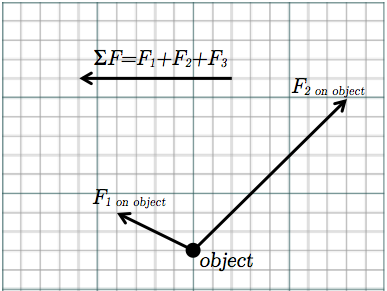
\includegraphics[height=150pt]{fnt612-4-vectors}
%	\vspace{-10pt}
%\end{wrapfigure}

\noindent Vectors $\vec{F}_\text{1 on object}$, $\vec{F}_\text{2 on object}$, and $\vec{F}_\text{3 on object}$ are all exerted on an object, adding together to form a net force vector, $\Sigma \vec{F}$, as shown in the graph to the right. However, only vectors $\vec{F}_\text{1 on object}$, $\vec{F}_\text{2 on object}$, and $\Sigma \vec{F}$ are known.\\

\noindent On a separate piece of graph paper, use the properties of vector addition to graphically determine the vector $\vec{F}_\text{3 on object}$.
\end{FNTenv}


\note{for \FNT~\thechapter-\ref{fnt6.1.2-5} }{
$\vec{F}_{1} = (-4, 4)$; $\vec{F}_{2} = (-14, 0)$
\\[0.25in]
Answer should be found graphically:
Solution: $\vec{F}_{3} $ = (0, -4); $\vec{F}_{4} $ = (18, 0); 
}\begin{FNTenv}
	\label{fnt6.1.2-5}

%\missingfigure{Needs a grid showing F1 and F2.}

\begin{wrapfigure}{R}{0.5\textwidth}
	\vspace{-32pt}
	\begin{center}
	\begin{tikzpicture}[thick,scale=0.65, every node/.style={transform shape},background rectangle/.style={fill=white}, show background rectangle]
		% draw a 10x7.5 grid in light gray with 5mm grid spacing
		\draw[step=.5cm,gray,very thin] (0,0) grid (10,7.5);
		% draw a darker grid in light gray with 2.5mm grid spacing
		\draw[step=2.5cm,gray,thick] (0,0) grid (10,7.5);
    
		% draw object node
		\draw (8.5,2.5) node[circle,minimum size=12pt,fill,inner sep=1pt]{} node[below=3pt]{object};
    
		% draw the first arrow, with descriptor F1; "Stealth" is the name of the arrowhead, and it's capitalized, so that it's scalable
		\draw[-{Stealth[scale=1.2]}, line width=1.5pt] (8.5,2.5) -- (6.5,4.5) node[above=6pt,align=center] {$\vec{F}_\text{1 on object}$};
    
		% draw the second arrow, with descriptor B
		\draw[-{Stealth[scale=1.2]}, line width=1.5pt] (8.5,2.5) -- (1.5,2.5) node[above=6pt]{$\vec{F}_\text{2 on object}$};
		
		% label "no net force" and forces to find
		\draw (2,5) node[above=3pt, align=left]{$\Sigma \vec{F} = 0$
								\\$\vec{F}_\text{3 on object}=?$
								\\$\vec{F}_\text{4 on object}=?$};
	\end{tikzpicture}
	\end{center}
	\vspace{-12pt}
\end{wrapfigure}

\noindent Vectors $\vec{F}_\text{1 on object}$, $\vec{F}_\text{2 on object}$, $\vec{F}_\text{3 on object}$, and $\vec{F}_\text{4 on object}$ are all exerted on an object, adding together to form a net force vector $\Sigma \vec{F} = 0$, as shown to the right.

However, only vectors $\vec{F}_\text{1 on object}$, $\vec{F}_\text{2 on object}$, and  $\Sigma \vec{F}$ (which is zero) are known. It is known that $\vec{F}_\text{3 on object}$ is completely vertical, and $\vec{F}_\text{4 on object}$ is completely horizontal.\\

\noindent On a separate piece of graph paper, use the properties of vector addition to determine the magnitudes of the vertical vector $\vec{F}_\text{3 on object}$, and the horizontal vector $\vec{F}_\text{4 on object}$.
\end{FNTenv}

\WCD
\vspace{12pt}

\note{for \FNT~\thechapter-\ref{fnt6.1.2-6} }{
$\vec{F}_{1} = (4.33, 2.5)$; $\vec{F}_{2} = (0, 15)$;  
\\[0.25in]
Answer should be found using trigonometry:
Solutions: \\
a) $\Sigma \vec{F} $ = (4.33, 17.5)\\
b) $\Sigma \vec{F} $ = 18.0 \@ 76.1$^{\circ}$
}
\begin{FNTenv}
	\label{fnt6.1.2-6}

%\missingfigure{Needs xy-axes showing F1 and F2}

\begin{wrapfigure}{R}{0.25\textwidth}
	\vspace{-39.5pt}
  	\centering
	\begin{center}
	\begin{tikzpicture}[thick,scale=0.65, every node/.style={transform shape},background rectangle/.style={fill=white}, show background rectangle]
		% draw xy-axes
		\draw[-{Stealth[scale=1.2]}, line width=0.5pt] (0,-0.5) -- (0,5) node[left=6pt,align=center] {$y$};
		\draw[-{Stealth[scale=1.2]}, line width=0.5pt] (-0.5,0) -- (3,0) node[below=6pt,align=center] {$x$};
		
		% draw F1
		\draw[-{Stealth[scale=1.2]}, line width=1.5pt] (0,0) -- (1.15,0.67) node[above=3pt,align=center] {$\vec{F}_1$};
		% Label F1 = 5N
		\node[label={[rotate=30]above:\unit[5]{N}}] at (0.577,0.333) {};
		% draw F1 arc
		\draw[line width=0.5] (0.6,0) arc (0:30:0.6);
		% label F1 arc 30deg
		\node[label={above:30\textdegree}] at (1.25,-0.25) {};
		
		% draw F2
		\draw[-{Stealth[scale=1.2]}, line width=1.5pt] (0,0) -- (0,4) node[right=6pt,align=center] {$\vec{F}_2$};
		% label F2
		\node[label={[rotate=90]left:\unit[15]{N}}] at (-0.125,2.5) {};
		
		% draw and label v_i
		\draw[->] (1.5,3) -- (2.5,3);
		\node[label={center:$\vec{v}_i=\unitfrac[3]{m}{s}$}] at (2,2.5) {};
	\end{tikzpicture}
	\end{center}
\end{wrapfigure}

\noindent Two force vectors ($\vec{F}_1$ and $\vec{F}_2$, as shown to the right) act on a \unit[2]{kg} object that has an initial velocity $\vec{v}_i$ of \unitfrac[3]{m}{s} in the $+x$-direction.

\begin{enumerate}[(a)]
	\item Use trigonometry to find the $x$- and $y$-components of the net force.
	\item Find the magnitude and direction of the net force.
\end{enumerate}
\end{FNTenv}

\WCD
\vspace{12pt}
\newpage

\note{for \FNT~\thechapter-\ref{fnt6.1.2-7} }{
a) Solution:  velocity vectors should be same magnitude pointing in the direction the cart is moving (so 2 equal and opposite velocity vectors)
b) Solution: Because cart 1 is half the mass of cart 2, the momentum vector for cart 1 should be half the magnitude of cart 2�s momentum vector. They should point in the direction the carts are moving respectively. Check to see that the student has drawn a picture and defined which way the carts are moving.
c) Check to see that students added the vectors tip to tail and that $p_{total}$ is not equal to 0.   
}
\begin{FNTenv}
	\label{fnt6.1.2-7}

Two rolling carts are moving toward each other at the \textbf{same speed}.  Cart 1 has a mass $m_1 = \unit[200]{g}$ and Cart 2 has a mass $m_2 = \unit[400]{g}$.

\begin{enumerate}[(a)]
	\item Draw a velocity vector $\vec{v}$ for each cart.
	
	\item Momentum $\vec{p}$ is a vector defined as $\vec{p} = m\vec{v}$.  Draw a momentum vector for each cart.
	
	\item Add the two momentum vectors together to find the total momentum, $\vec{p}_\text{total} = \vec{p}_1 + \vec{p}_2$.
\end{enumerate}
\end{FNTenv}

\WCD
\vspace{12pt}

\note{for \FNT~\thechapter-\ref{fnt6.2.1-1} }{
Go over student questions. Students were to rework parts of \hyperref[act6.2.1]{Activity~\ref{act6.2.1}} on page \pageref{act6.2.1} (spring scale activity) they found confusing.  
}
\begin{FNTenv}
	\label{fnt6.2.1-1}

Rework the parts of Activity \ref{act6.2.1} that you still have questions about. Bring any remaining questions to the next DL meeting.
\end{FNTenv}

\WCD